\documentclass[12pt, twoside]{report}

\usepackage[a4paper, margin=1.5cm]{geometry}

\usepackage{minted}
\setminted[python]{autogobble=true}
\usemintedstyle{xcode}

\usepackage{titlesec}
\titlespacing*{\chapter}{0pt}{20pt}{20pt}
\titleformat{\chapter }[display]{\normalfont\huge\bfseries}{\chaptertitlename\
\thechapter}{20pt}{\Huge}

\usepackage{graphicx}
\usepackage{hyperref}

\usepackage{amsmath}
\usepackage{amssymb}
\usepackage{amsthm}

\theoremstyle{plain}
\newtheorem{theorem}{Theorem}[chapter]
\theoremstyle{definition}
\newtheorem{definition}{Definition}[chapter]
\newtheorem{corollary}{Corollary}[theorem]
\theoremstyle{definition}
\newtheorem{example}{Example}[chapter]

\providecommand{\abs}[1]{\lvert#1\rvert}
\providecommand{\norm}[1]{\lVert#1\rVert}

\begin{document}


% The 'article' document class provides a simple way to make a title
% page: 

\title{
    \large{Numerical Solution to the Initial Value Problem by a 
    Predictor-Corrector Method:}\\
    Applications to n-Body Problem and Pendula}
\author{Joel Biffin}
\maketitle

% A table of contents can be generated automatically as well:

\tableofcontents


\begin{abstract}

    Initial Value Problems primarily arise from the modelling of natural
    phenomena where often we are able to desribe some quantity's rate of change
    as a function of itself coupled with time. This report will focus on
    Initial Value Problems arising from models using Ordinary Differential
    Equations. It is notable that many of the breakthroughs in the field of
    solving Partial Differential Equations have arisen from spacially
    discretising the problem and approximating solutions to the discretised
    Initial Value Problem.

    Leibniz and Newton are often cited as the fathers of the field of
    differential equations. Similar to Newton, in this report we will be
    considering quantities which change with respect to time, but all of the
    methods and analyses apply for any other variable too. 

    Until the late 19th century, numerical algorithms to approximate solutions
    to Initial Value Problems could not usefully be applied. Since then
    contributions from Adams, Milne, Butcher and Gear (to name a few) have been
    used in computations an unimaginable number of times as a result of now 
    readily available computing power. 

    In this report, established methods will be analysed and reviewed 
    comparatively in terms of implementation complexity, computational cost
    and accuracy.

\end{abstract}


% Now comes the true content. 

\chapter{Background}
    
    \section{Notation}
    \label{1_notation}
        Throughout this report, vector quantities and functions will be written
        in lowercase bold type ($\mathbf{u}, \mathbf{f}$), scalar quantities 
        and functions will be written in lowercase type ($t, f$), and iterative
        schemes will use subscripting to represent the $i$-th iteration 
        ($u_{i}, \mathbf{u}_i$) of a method. Generally, vector quantities will
        be expressed as such rather than element-wise, unless otherwise stated.


    \section{Initial Value Problems}
    \label{1_ivp}
        An Initial Value Problem (IVP) can generally be written in the form,
        \begin{equation}
        \label{eq:ivp}
            \begin{split}
                \frac{d \mathbf{u}(t)}{dt}& = \mathbf{f}(t, \mathbf{u}), 
                \quad t \in [a, b]\\
                \mathbf{u}(a)& = \mathbf{u}_0, \quad \text{(given)},
            \end{split}
        \end{equation}
        using vector quantities. It is worth noting that this is in the form of
        a 1st order system of differential equations, this is due to the fact 
        we can reduce any $n$-th order equation to a system of first order ones
        (see section ).


    \section{Where Do They Come From?}
    \label{1_origins}
        As discussed in the abstract, IVPs often arise from, but are not
        restricted to, the modelling of natural phenomena. 

        Newton's 2nd Law of Motion describes the proportionality of the rate 
        of change of velocity to the resultant force acting on a body. This 
        coupled with an initial condition $\mathbf{v}(a)=\mathbf{v}_0$, gives
        an IVP. In electrical circuit modelling, the flow of charge $q$ from a
        capacitor of known initial charge $q(0)=q_0$ can too be modelled by an 
        IVP in the form of \eqref{eq:ivp}.


    \section{Existence \& Uniqueness of Solutions}
    \label{1_existence}
        Before discussing methods used to approximate solutions to IVPs, it is
        important to ascertain whether solutions do in fact exist and, if so,
        whether or not they are unique. We will use Lipschitz continuity to do
        so.
        \begin{theorem}
            Let $f(t,u)$ be a continuous function for all $u$ and $t \in 
            [a, b]$, and suppose that $f$ satisfies the Lipschitz condition,
            \begin{equation}
            \label{eq:lipschitz}
                \abs{f(t,v)-f(t,w)} \le L\abs{v-w},
                \quad \forall v, w \text{ and } t \in [a,b].
            \end{equation}
            Then, for any $u_0$ there exists a unique continuously
            differentiable function $u(t)$ defined on $[a,b]$ satisfying
            \eqref{eq:ivp}.
        \end{theorem}
        This result is incredibly important when modelling environments and 
        phenomena. If a model equation does not satisfy our Lipschitz condition
        this is a real indicator of whether or not our model correctly 
        represents our system.

        For the remainder of this report we will be concerned with problems 
        which do satisfy our Lipschitz condition \eqref{eq:lipschitz}.


    \section{Analytical Methods vs Numerical Methods}
    \label{1_analytical_numerical}
        Analytical methods can be used to solve IVPs but only for a very limited
        number of special cases. In terms of computing, there are a number of 
        software packages that are able to solve these differential equations
        symbolically (for example, MATLAB's `MuPAD'). Since it is the case that
        the majority of ordinary differential equations cannot by solved 
        analytically, these algorithms are of little use (and it's worth noting
        that these algorithms are notoriously costly).

        This inability to analytically find solutions led to the discussion of
        numerical methods to approximate solutions to IVPs at a specific $t$. 
        The general approach for these numerical methods begins with 
        discretising our independent variable $t$ into a mesh. This mesh is an 
        increasing monotonic sequence of time values ${\lbrace 
        t_i\rbrace}_{i=0}^n$, where $[a,b]$ has been split into $n$ (not 
        necessarily equally spaced) intervals such that $a=t_0$ and $b=t_n$.

        In practice, numerical methods are the best approach to finding 
        solutions to IVPs and when used appropriately they produce incredibly 
        useful results to equations that we would otherwise be unable to solve.

        In the next chapter we will be discussing what it is that makes a 
        numerical algorithm appropriate for a given problem. We will also be
        investigating the accuracy of our approximations.



\chapter{Numerical Methods}

    Algorithms which approximate solutions to \eqref{eq:ivp} fall into three
    categories: Taylor Series methods, Linear Multistep Methods (LMMs) and 
    Runge-Kutta methods. It can be viewed that all three of these families are
    generalisations of Euler's Method (\ref{2_forward_euler}). 

    The focus of this project primarily lies with Linear Multistep Methods and 
    using them in the form of a predictor-corrector pair. Runge-Kutta methods
    are too used and evaluated here, but are only featured in case studies
    as starting schemes for LMMs.

    For the purposes of software design we have classified Euler's Method as a
    One-Step method, and similarly Runge-Kutta methods are classified as 
    One-Step methods too. Unless explicitly stated, all methods will use a 
    fixed step-size $h=\frac{b-a}{n}$ (where $n$ is the number of time 
    intervals) producing an equally spaced mesh.

    \section{One-Step Methods}
    \label{2_onestep}
        
        \subsection{(Forward) Euler's Method}
        \label{2_forward_euler}
            Euler's method is given by the iterative scheme,
            \begin{equation}
            \label{eq:euler}
                \mathbf{u}_{i+1} = \mathbf{u}_i + h\mathbf{f}(t_i, 
                \mathbf{u}_i).
            \end{equation}
            This scheme is \textit{explicit} since we can calculate 
            $\mathbf{u}_{i+1}$ using a combination of $\mathbf{u}_i$ and $t_i$
            which are known at the start of an iteration.

            \begin{definition}
                An iterative scheme is called \textbf{explicit} if at the 
                beginning of an iteration we can express $\mathbf{u}_{i+1}$ in 
                terms of values which have already been computed or can be 
                computed by simple substitution during the iteration. In 
                contrast, \textbf{implicit} schemes have $\mathbf{u}_{i+1}$ 
                appearing on both `sides' of our scheme, so an algebraic 
                equation must be solved at each iteration to compute 
                $\mathbf{u}_{i+1}$.
            \end{definition}

            We will discuss later on how the explicit nature of a method 
            impacts its stability.

        \subsection{(Backward) Euler's Method}
        \label{2_backward_euler}
            This method can be viewed as an \textit{implicit} variant of 
            \eqref{eq:euler}, and is given by
            \begin{equation}
            \label{eq:backward_euler}
                \mathbf{u}_{i+1} = \mathbf{u}_i + h\mathbf{f}(t_{i+1}, 
                \mathbf{u}_{i+1}).
            \end{equation} 
            Since $\mathbf{u}_{i+1}$ appears on both sides of our expression,
            we must solve
            \begin{equation}
            \label{eq:nonlinear_equation}
                \mathbf{g}(\mathbf{u}_{i+1}) = \mathbf{u}_{i+1} - 
                \mathbf{u}_i - h\mathbf{f}(t_{i+1}, \mathbf{u}_{i+1}) 
                = \mathbf{0}
            \end{equation}
            for $\mathbf{u}_{i+1}$ at every iteration.

            Of course, we could solve this symbolically at a cost, but in
            practice we use any numerical (vector) root finding algorithm 
            (Secant Method, Newton's Method etc.). 

            Originally in this project Newton's Method was applied using the 
            \mintinline{python}{scipy.optimize.newton} package in Python where 
            the Jacobian matrix was approximated via Finite Differences. As is 
            conventional, the initial `guess' solution was computed via 
            \eqref{eq:euler}. Unfortunately this method led to some 
            non-convergent solutions being returned. Eventually the decision 
            was made to use the \mintinline{python}{scipy.optimize.fsolve} 
            package which implements a variant of the Powell hybrid method.


    \section{Global \& Local Truncation Error}
    \label{2_error}
        As with any numerical approximations, our methods will introduce 
        errors. Here we will include floating point errors in our
        truncation error considerations, so floating point errors are not
        noted directly but are considered in implementation.

        \begin{definition}
            The \textbf{Global Truncation Error} (GTE), denoted $e_{i}(t)$,
            is the total error in our approximation. It is given by 
            $e_i=u(t_i) - u_i$, where $i$ represents the $i$-th iteration
            in the standard way (see Subsection \ref{1_notation}).
        \end{definition}

        \begin{definition}
            The \textbf{Local Truncation Error} (LTE), denoted $\tau (h)$,
            for a numerical method is the error introduced in one single 
            iteration. This is the error introduced in computing 
            $\mathbf{u}_{i+1}$ when all previously computed values are taken 
            to be exact.
        \end{definition}

        GTE is really just a consequence of LTE and due to this it is helpful
        to address our full attention to the analysis of LTE.
        
        For any method we can derive an expression for the order of LTE by 
        using a Taylor Series expansion for the exact solution to the ODE and
        take the difference between that and our iterative scheme (when all 
        previous values are taken to be exact). Doing this for Euler's method 
        is shown:
        
        Suppose $u_i = u(t_i)$, then Euler's method gives us, 
        \begin{equation}
            \begin{split}
                u_{i+1} &= u(t_i) + hf(t_i, u(t_i)) \\
                &= u(t_i) + hu'(t_i),\quad
                \text{since } u'(t_i) = f(t_i, u(t_i)).
            \end{split}
        \end{equation}
        Our Taylor expansion for our exact solution is,
        \begin{equation}
            u(t_{i+1}) = u(t_i + h) = u(t_i) + hu'(t_i) + \frac{h^2}{2} 
            u''(\xi_i) + O(h^3), \quad \xi_i \in (t_i, t_{i+1}).
        \end{equation}
        Taking the difference of these two expressions leaves us the remainder,
        \begin{equation}
            \tau(h) = u(t_{i+1}) - u_{i+1} = \frac{h^2}{2} u''(\xi_i) + 
            O(h^3) = O(h^2),
        \end{equation}
        so we know that for Forward Euler we have $\tau(h)=O(h^2)$.

        It's worth noting that a similar process can be carried out to find an expression for GTE but without the assumption that 
        $u_i=u(t_i)$. 
        \begin{definition}
            A method is said to be of \textbf{order} $p$ if its LTE satisfies 
            $\tau(h)=O(h^{p+1})$. If $p \ge 1$ then we say that the method is
            consistent of order $p$.
        \end{definition}
        With this definition we know that Forward Euler is an order 1 method 
        -- so too is Backward Euler. In addition, when our method is order $p$,
        we know that the GTE, $e_i=O(h^p)$ too.


    \section{Convergence \& Stability}
    \label{2_stability}
        Efforts in using these numerical algorithms would be fruitless if the 
        results obtained were not representative of the \textit{true} solution.
        So it is important that we know a method is \textit{convergent} before 
        using it.

        \begin{definition}
            A method is said to be \textbf{0-stable} if a small perturbation 
            $\boldsymbol{\varepsilon}$ ($\norm{\boldsymbol{\varepsilon}} 
            << 1$) to $\mathbf{u}_0$ causes the numerical solution to change 
            at most by $K\boldsymbol{\varepsilon}$, where $K$ is independent 
            of $h$.
        \end{definition}

        We will later discuss the \textit{root condition} which can be used as
        a quantitative method to establish 0-stability, but for the moment this
        qualitative definition is all we need.

        \begin{theorem}[Dahlquist's Equivalence Theorem]
        \label{2_dahlquist}
            A numerical method is said to be convergent of order $p$ if and 
            only if it is 0-stable and consistent of order $p$.
        \end{theorem}

        \begin{corollary}
        \label{2_dahlquist_corollary}
            A convergent numerical method has the property that,
            \begin{equation}
                \lim_{h \to 0} \norm{\mathbf{u}(t_i) - \mathbf{u}_i} = 0.
            \end{equation}
        \end{corollary}

        In practice, we are computing with floating point numbers so, in an 
        arbitrary precision, by taking $h$ to be excessively small then the 
        accuracy that we might theoretically gain will be counteracted by round-off errors.
        

        \subsection{Absolute Stability}
        \label{2_absolute_stability}
            Given that a method is \textit{0-stable} we know that if we take 
            $h$ to be sufficiently small we acheive a very good representation
            of the true solution. But how small does $h$ have to be? Are there any limitations on how \textit{large} $h$ is?

            Consider the scalar \textit{test equation},
            \begin{equation}
            \label{2_test_equation}
                u' = \lambda u, \quad \lambda \in \mathbb{C},
            \end{equation}
            whose solution is known, $u(t)=c e^{\lambda t}$ for some constant 
            $c$. When $\mathbb{R}\text{e}\{\lambda\} < 0$, our solution 
            converges to 0 as $t\to\infty$. This results in the absolutely 
            decreasing sequence of approximations 
            ${\lbrace u_i \rbrace}_{i=0}^{\infty}$.

            We want our numerical methods to share this property when acting 
            on the test equation.

            \begin{definition}
                The \textbf{region of absolute stability} is the set of 
                $h\lambda\in\mathbb{C}$ where 
                ${\lbrace u_i \rbrace}_{i=0}^{\infty}$ is an absolutely
                decreasing sequence.
            \end{definition}

            We can find the region of absolute stability by applying our 
            numerical method to the test equation. For forward Euler we attain 
            the region $\abs{1+h\lambda} \le 1$ which provides us a very 
            restrictive upper bound on the value of $h$ we can choose. 
            Applying backward Euler gives the region 
            $\abs{1-h\lambda}^{-1} \le 1$, which is satisfied for all values 
            of $h, \lambda$ where $\mathbb{R}\text{e}\{\lambda\} \le 0$.
            Hence the entire left half-plane is in the region of stability and there is no restriction on the value of $h$ we can choose.

            \begin{definition}
                A numerical method having the full left-half plane in its region of absolute stability is said to be \textbf{A-stable}.
            \end{definition} 


        \subsection{Stiffness}
        \label{2_stiffness}
            Ideally we would be able to choose our step size $h$ based solely
            on the accuracy we want from our computation. Unfortunately this is
            not always the case -- as highlighted by our region of absolute
            stability for forward Euler. The \textit{stiffness} of a system helps characterise this problem.

            \begin{definition}
                An IVP is said to be \textbf{stiff} if the step size required 
                to satisfy our absolute stability requirement is significantly smaller than the step size required to approximate at some desired accuracy.
            \end{definition}

            \begin{example}
                Consider the IVP,
                \begin{equation}
                \label{eq:2_stiff_ex}
                    \begin{cases}
                        u'(t) = 100u(t), \quad \text{on } t \in [0,0.2],\\
                        u(0) = 10.
                    \end{cases}
                \end{equation}
                Figure \ref{2_stiff_graphs} demonstrates the impact of our 
                equation's stiffness on our results using forward Euler. By 
                method of substitution, our absolute stability expression 
                tells us that in order to compute stable approximations using 
                \eqref{eq:euler} we must use $h \le 0.02$. In contrast, we 
                have no bound on our choice of $h$ in terms of stability for 
                backward Euler. This is highlighted by the general shape of 
                our graphs in comparison to results from forward Euler.

                \begin{figure}
                    \centering
                        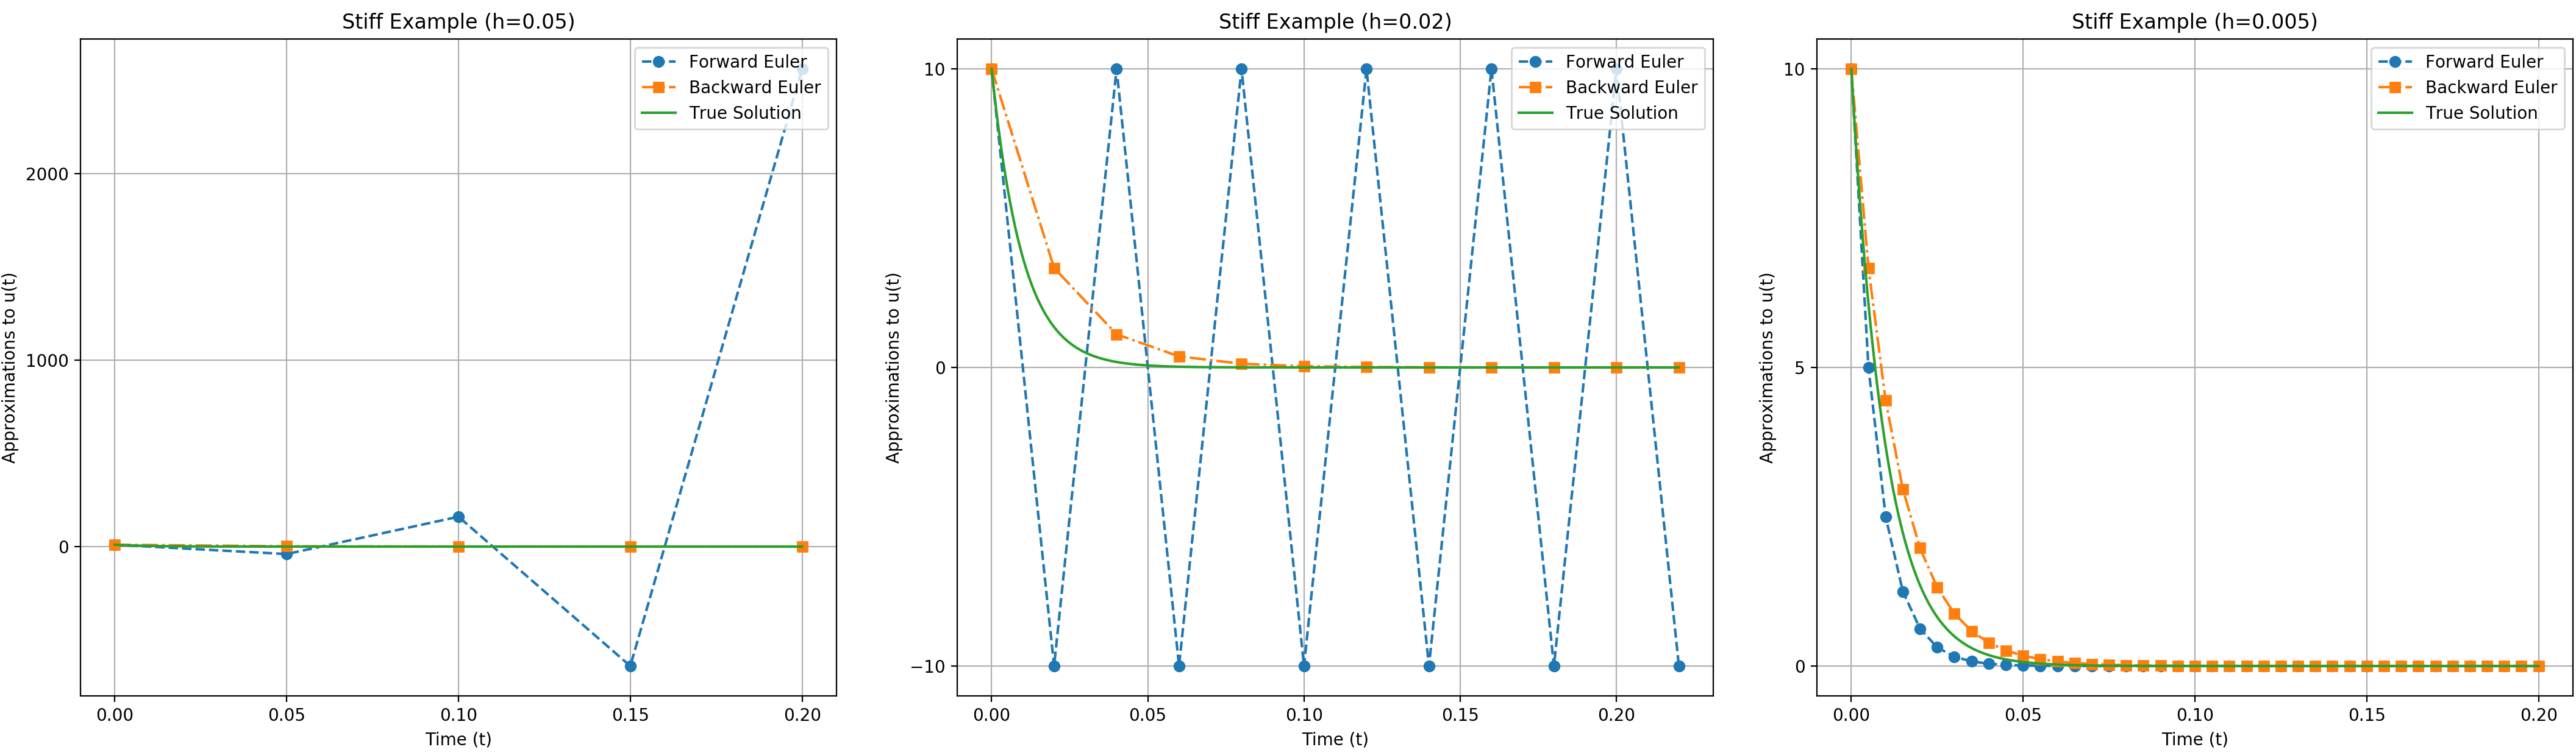
\includegraphics[width=\columnwidth]{stiff_graphs}
                        \caption{Demonstration of stiffness using 
                        \eqref{eq:euler} \& \eqref{eq:backward_euler}
                        with $h=0.05, 0.02, 0.005$ on \eqref{eq:2_stiff_ex}}
                        \label{2_stiff_graphs}
                \end{figure}
            \end{example}

            In summary, we must be careful when choosing numerical methods to 
            solve stiff equations. Depending on the stiffness, we must decide 
            between the performance of choosing an explicit method with 
            smaller steps or using an implicit method with larger steps, but 
            needing to numerically solve an equation such as 
            \eqref{eq:nonlinear_equation} at each iteration.

    \section{Runge-Kutta Methods}
    \label{2_runge_kutta}
        Runge-Kutta methods (first discussed by Runge 1895) look to solve the 
        problem of \textit{how can we improve the accuracy of our 
        approximations without the need to take significantly smaller time 
        intervals?}. Here we won't discuss Runge-Kutta methods in much depth 
        as it is outside of the scope of this project, but we will mention 
        asymptotic complexity and derivations.

        From attempting to integrate \eqref{eq:ivp}, we can apply a Gauss quadrature rule,
        \begin{equation}
        \label{eq:fundamental_theorem_calculus}
            \mathbf{u}_{i+1} = \mathbf{u}_i + \int_{t_i}^{t_{i+1}} 
            \mathbf{u}'(t) dt,
        \end{equation}
        to solve our differential equation. It is with this idea that Runge-Kutta methods were established.

        The general notion is that if we can evaluate intermediate values 
        (or \textit{stages}) between $\mathbf{u}_i$ and $\mathbf{u}_{i+1}$, we can better approximate $\mathbf{u}_{i+1}$. 

        \subsection{4-Stage Runge-Kutta}
        \label{2_rk4}
            Generally the most popular Runge-Kutta method is known as the 
            \textit{Classical Runge-Kutta} which is in fact a special case of 
            the generalised 4-stage Runge-Kutta. The generalised form has $10$
            free parameters, optimising these parameters to yield the highest 
            possible \textit{order} gives us our `Classical' method. This 
            method is given by the iterative scheme,
            \begin{equation}
            \label{eq:rk4}
                \begin{split}
                    \mathbf{u}_{i+1} &= \mathbf{u}_i + 
                    \frac{h}{6} (\mathbf{k}_1 + 2\mathbf{k}_2 + 2\mathbf{k}_3 
                    + \mathbf{k}_4), \quad 
                    \text{where }\\
                    \mathbf{k}_1 &= \mathbf{f}(t_i, \mathbf{u}_i),\\
                    \mathbf{k}_2 &= \mathbf{f}(t_i+\frac{h}{2}, 
                    u_i+\frac{1}{2}\mathbf{k}_1),\\
                    \mathbf{k}_3 &= \mathbf{f}(t_i+\frac{h}{2}, 
                    \mathbf{u}_i+\frac{1}{2}\mathbf{k}_2),\\
                    \mathbf{k}_4 &= \mathbf{f}(t_i+h, 
                    \mathbf{u}_i+\mathbf{k}_3).
                \end{split}
            \end{equation}
            This method is fourth order as $\tau(h)=O(h^5)$. 

            In practice, Runge-Kutta methods have great accuracy properties
            and for small examples often yield sufficient results at a 
            reasonable time cost. Their downsides however, are in the fact
            that every iteration we are computing a number of intermediate
            values and then discarding them after each iteration. These 
            intermediate function evaluations actually dominate our 
            algorithm's running time. Consequently, when working on large 
            systems of complicated ODEs our computations become very 
            inefficient. 

    \section{Linear Multistep Methods}
    \label{2_lmms}
        In a similar vein to Runge-Kutta methods, Linear Multistep Methods 
        look to use more information from $t<t_{i+1}$ to improve our 
        approximations. In contrast to Runge-Kutta methods, LMMs use 
        previously computed values in their schemes which helps to avoid the problem highlighted at the end of Section \ref{2_runge_kutta}.

        Unlike aforementioned one-step methods, LMMs are not 
        \textit{self-starting} and in order to carry out the first steps, a 
        starting scheme must be decided on. Often a Runge-Kutta method of
        appropriate order is used as a starting routine. This method is chosen
        to have an order equal to or higher than the coupled LMM, to preserve
        asymptotic accuracy.

        \subsection{Adams Methods}
        \label{2_adams}
            Adams methods were devised in the late 19th century (prior to 
            Runge). They are derived from trying to solve the integral 
            equation,
            \begin{equation}
            \label{2_int_equation}
                \mathbf{u}(t_{i+1}) = \mathbf{u}(t_i) + \int_{t_i}^{t_{i+1}}
                \mathbf{f}(t, \mathbf{u}(t)) dt,
            \end{equation}
            by approximating our integrand by a polynomial which interpolates
            our previously computed $\mathbf{u}_j$ values.

            A $k$-step \textit{Adams-Bashforth} method is an \textit{explicit}
            Adams scheme which interpolates to $k$ values to approximate 
            our integrand, $\mathbf{f}(t, \mathbf{u}(t))$. A $k$-step method 
            has LTE of $\tau(h)=O(h^{k+1})$, so is order $k$. It's worth 
            noting that over the bounds of our integral, $(t_i, t_{i+1})$, we 
            are \textit{extrapolating} which is often unreliable.

            The $2$ and $3$-step Adams-Bashforth methods are given by their 
            iterative schemes,
            \begin{align}
                \mathbf{u}_{i+1} &= \mathbf{u}_{i} + \frac{h}{2} 
                (3\mathbf{f}(t_i, \mathbf{u}_i) - 
                \mathbf{f}(t_{i-1},\mathbf{u}_{i-1})),\\
                \mathbf{u}_{i+1} &= \mathbf{u}_{i} + \frac{h}{12} 
                (23\mathbf{f}(t_i, \mathbf{u}_i) - 
                16\mathbf{f}(t_{i-1},\mathbf{u}_{i-1}) + 
                5\mathbf{f}(t_{i-2}, \mathbf{u}_{i-2})).
            \end{align}

            Implicit Adams schemes are known as \textit{Adams-Moulton} 
            methods. They are derived in a similar way to Adams-Bashforth 
            methods except a $k$-step \textit{Adams-Moulton} method looks to 
            approximate the integrand with a polynomial which interpolates to 
            $k+1$ points. This results in integrating over an interpolated 
            region which is much more reliable than the explicit schemes. 

            The trade-off for this increase stability is that we must solve
            a non-linear equation (similar to \eqref{eq:nonlinear_equation}) at
            every iteration -- which we know is costly.

            The $1$ and $2$-step Adams-Moulton methods are given by their iterative schemes,
            \begin{align}
                \mathbf{u}_{i+1} &= \mathbf{u}_{i} + \frac{h}{2} 
                (\mathbf{f}(t_i, \mathbf{u}_i) + 
                \mathbf{f}(t_{i+1},\mathbf{u}_{i+1})),\\

                \mathbf{u}_{i+1} &= \mathbf{u}_{i} + \frac{h}{12} 
                (5\mathbf{f}(t_{i+1}, \mathbf{u}_{i+1}) +
                8\mathbf{f}(t_{i},\mathbf{u}_{i}) -
                \mathbf{f}(t_{i-1}, \mathbf{u}_{i-1})).
            \end{align}


        \subsection{Nystrom Methods}
        \label{2_nystrom}

        \subsection{Backwards Differentiation Formulae}
        \label{2_bdf}


    \section{Predictor-Corrector Methods}
    \label{2_predictor_correctors}


    \section{Adaptive Step-Size}
    \label{2_adaptive}

\begin{thebibliography}{50}
    \bibitem{ascher}
        U.M.~Ascher, L.R.~Petzold,
        ``Computer Methods for Ordinary Differential Equations and 
        Differential-Algebraic Equations'',
        Philadelphia: SIAM (1935).

    \bibitem{newton}
        I.~Newton,
        ``Philosophiae Naturalis Principia Mathematica (“Mathematical
        Principles of Natural Philosophy”)'' London (1687).

    \bibitem{hairer}
        E.~Hairer, S.P.~N{\o}rsett, G.~Wanner,
        ``Solving Ordinary Differential Equations I'',
        Springer-Verlag Berlin Heidelberg (1993).

    \bibitem{higham}
        D.F~Griffiths, D.J~Higham,
        ``Numerical Methods for Ordinary Differential Equations'',
        Springer-Verlag London Limited (2010).

    \bibitem{powell}
        ``https://www.math.utah.edu/software/minpack/minpack/hybrd1.html'', 
        ``Documentation for MINPACK subroutine HYBRD1'',
        April 2019.

    \bibitem{suli}
        E.~Suli, D.~Mayers,
        ``An Introduction to Numerical Analysis'',
        Cambridge University Press (2003).

    \bibitem{gregory}
        R.D.~Gregory,
        ``Classical Mechanics'',
        Cambridge University Press (2006).


\end{thebibliography}

\end{document}
